%%Below is the guy I stole this template from, because it is great
%%%%%%%%%%%%%%%%%%%%%%%%%%%%%% -*- Mode: Latex -*- %%%%%%%%%%%%%%%%%%%%%%%%%%%%
%% uhtest-body.tex -- 
%% Author          : Robert Brewer
%% Created On      : Fri Oct  2 16:30:37 1998
%% Last Modified By: Robert Brewer
%% Last Modified On: Mon Oct  5 16:01:29 1998
%% RCS: $Id: uhtest-body.tex,v 1.1 1998/10/06 02:07:14 rbrewer Exp $
%%%%%%%%%%%%%%%%%%%%%%%%%%%%%%%%%%%%%%%%%%%%%%%%%%%%%%%%%%%%%%%%%%%%%%%%%%%%%%%
%%   Copyright (C) 1998 Robert Brewer
%%%%%%%%%%%%%%%%%%%%%%%%%%%%%%%%%%%%%%%%%%%%%%%%%%%%%%%%%%%%%%%%%%%%%%%%%%%%%%%
%% 



%%%%%%%%%%%%%%%%%%%%%%%
\chapter{Introduction}
%%%%%%%%%%%%%%%%%%%%%%%

Every dissertation should have an introduction.  You might not realize
it, but the introduction should introduce the concepts, background,
and goals of the dissertation.

\section{Cosmological Theory}
	\subsection{Cosmic Rays}
		The universe is vast and surprising and has just begun to be explored.  As telescopes become larger and more sensitive, we as a species can see further and further away from our tiny blue speck.  However, the attenuation of photons in space from fundamental physics interactions clouds the majority of the universe from our gaze.  In addition, there is a constant flux of bosonic particles incident on earth from various cosmic accelerators.  These messenger particles allow a new window into regions of the universe that were previously inaccessible.  The energy spectrum of these particles introduces an additional mystery, as the sources and interactions of these particles isn't entirely understood.  The makeup of these particles is also poorly understood, whether it be heavy ions or protons.  Additional experimental observations of cosmological particles incident to the earth will yield a better understanding of both the makeup of the matter within the universe, as well as fundamental physics information unavailable from existing collider experiments.  The creation and propagation of ultra high energy cosmic rays through the universe open a window to extreme high energies.
	\subsection{History}
		Cosmic rays were first observed a century ago, when an unexpected increase in observed bosonic radiation was observed as altitude increased.  Previously, it was expected that radiation was caused by radioactive decays within the earth's crust, however this additional radiative component was indicative of a cosmological source.
	\subsection{Sources}
		There are numerous sources that have strong theoretical motivation to create cosmic rays, and due to the higher flux of nearby low energy cosmic ray sources, additionally have some experimental evidence to support those theories.  They include such objects and Active Galactic Nuclei (AGN), supernova, quasars, gamma-ray bursts.  However these sources still have uncertainty, and their creation mechanisms may be much more complex than current models suppose.


\section{GZK internation}
		The flux of cosmic ray particles as a function of energy, the energy spectrum, decreases suddenly at a specific energy.  This energy coincides with the delta resonance energy of a relativistic particle and the cosmic microwave background radiation (CMB).  This interaction was predicted by Greisen–Zatsepin–Kuzmin, and represents a theoretical high energy limit on particles coming from outside of the galaxy, known as the GZK limit, at 5x10$^{19}$ eV.  Confoundingly, cosmic ray particles have been observed exceeding this limit, suggesting an intra-galactic source of unknown origin.  The low statistics of particles observed at this energy prevent identification of a specific source.  However, as particles are present at these high energies, it is expected that other regions of the universe also contain accelerators capable of creating cosmic rays in excess of the GZK limit.  The GZK process has multiple channels, neutral current and charged current, each of which produce ultra high energy neutrino messenger particles that can be detected on earth.

\subsection{Neutrino detection on earth}
		Cosmologically propagating neutrinos have an extremely small cross section, such that their path length through empty space is essentially infinite.  This yields a messenger particle that can transmit information about ultra high energy cosmic ray quantity, flux, and energy from regions of the universe not probe-able by classical photon telescopes.  Neutrino telescope observations have been carried out at lower energies for nearly a century, with a recent increase in energies and scale in the past few decades.  Since the term "cosmic ray" describes any high energy particle incident on earth (including gamma rays).  For the purposes of this dissertation, neutrinos fit the description of cosmic rays.
	\subsection{Neutrino hadronic interactions}
		Though neutrinos have a small cross-section with vacuum, they have a non-trivial cross-section with hadronic matter through the weak interaction.  Luckily, the earth where we reside is an enormous target for these low flux particles.  These interactions create a hadronic shower, one that radiates heavily.


%%%%%%%%%%%%%%%%%%%%%%%%%%
\chapter{ANITA Telescope}
%%%%%%%%%%%%%%%%%%%%%%%%%%
\section{Overview}
	The ANITA telescope platform is, in essence, a passive broad-band radio frequency electromagnetic field transient detector and time domain digitizer.  The main structure consists of a collection of radially positioned, outwardly facing, broad-band, highly-directional quad-ridge horn antennas.  The antennas are separated into three different rings, with each ring separated into 16 different "phi-sectors."  This yields several (2-3 for ANITA2, 3 for ANITA3) antennas pointing in the same direction with a physics baseline offset between them. These antennas' feeds are filtered and amplified by a series of low noise-figure signal-chain components, discussed later, before being digitized by custom on board high-speed digitizer chips and readout electronics.  The digitization is triggered on-board, with a separate square-law integrating power detector before being read out to on board redundant data storage.  The payload is capable of reading out ~50Hz of full payload waveforms with low (\textless 5\% ) deadtime to disk through a CPCI interconnect backplane.  Additional position and orientation data is also recorded, as well as multiple diagnostic and in-situ relevant physics measurements.	
	
\section{Quad Ridge Horn Antennas}
	The ANITA instrument utilizes dual polarized quad ridge horn antennas to convert the electromagnetic field incident to the payload into an electrical signal that can be digitized and stored for later analysis.  The main requirements of the antennas are: equal sensitivity over a large range of frequencies, high directionality in order to reduce noise from other RF power sources, dual polarizations with co-located phase centers, low dispersion, and light weight.  \\
	Antennas are located to maximize baseline distance between pairs pointing to similar regions of sky in order to maximize angular resolution recovered from interferometric pointing.  Each successive ANITA flight has added additional antennas to the nadir ring in order to increase the number of baselines, as well as provide an additional $\frac{1}{\sqrt{N}}$ noise reduction for coherently summed waveforms.  The total size of the antennas are dictated by the minimum desired frequency (f=1/$\lambda$), a term dominated by both physical payload constraints as well as anthropogenic CW noise.  Additionally, dual polarizations are required for the physics of the instrument, as the radiation emitted by particle interactions is expected to be radially polarized around the shower axis.  The polarization convolved with the refractive index of the ice will yield an entirely vertically polarized field transient at the payload for shower interactions within the ice, and an entirely horizontally polarized transient for showers above the ice.  The dispersion of the antennas must also be low as the digitization window is small and the square-law power trigger is dependent on all power being within its integration window. \\
	Calibrations of the antennas was performed over a wide range of angles in order to determine the full beam-pattern of the horns in both the E-field and B-field for each polarization.  These measurements were taken for the boresight of every antenna as well, in order to determine stability of the manufacturing process.  These variations are discussed later in the Calibration chapter.
	\subsection{Antenna Theory}
		Since this is my dissertation, I should probably talk a bit about antenna theory and antenna height and stuff like that.  I can either do that here or in the calibration section, but since I'm not very good at that stuff I'll wait.
	
\section{Filtering}
	\subsection{Importance}
		The radiative Askaryan signal has a very wide bandwidth, however there are a few considerations that require the signals read by the ANITA telescope to be limited to a specified bandwidth.  \\
		At the high frequency end of the spectrum, above 1.2GHz, the radiative particles in the shower begin to be resolvable, leading to a loss of coherence of the radiated power.  This is especially true at postions not at the Cherenkov angle from the shower axis.  The lack of coherent signal power in the UHV region, coupled with the increased noise induced from widening the band, advises a low-pass filter on the input of the system. \\
		On the low frequency end, the radiated power from the shower is expected to be both coherent and strong, however the physical limitations of building a long wavelength antenna coupled with the high utilization of the VHF band by radio transmitters on satellites and ground stations lead to a requirement that lower frequencies be removed. \\
	\subsection{Technical Details}
		This band pass filtering is done in two stages, one immediately after the antenna, before the pre-amplifier, in order to prevent saturation of the pre-amplifier from out of band signals.  This filter must have an extremely low in-band loss, as any loss introduced by the filter is gained in full system noise temperature, a value which is cascaded through the entire amplification chain.  This was accomplished with a custom made LARK band pass filter.  The second is done after the full amplification chain in order to remove the added out of band electronic amplifier noise introduced from the system.  This was accomplished with two separate low-pass/high-pass filters.
		
		
\section{Amplification}
	\subsection{Expected Power}
		The power of an Askaryan signal from the continent is proportional to the energy of the incident cosmic ray particle.  The 
	\subsection{Noise Figure} 
	The extremely low signal power of an Askaryan pulse necessitates a minimum of additional electronics noise from the detector.  Besides a background of thermal noise, the dominant continuous noise source is electronics noise from the amplifiers.  This noise is a byproduct of the non-ideal coupling of the amplifier to the input signal that results in the amplification of internal thermal noise seen as a resistance on the front of the amplifier.  The noise figure is increased by any loss of power in front of the amplifiers.  Since the noise figure cascades through an amplifier chain, it is imperative to reduce any additional noise figure at the front of the signal chain, and less important in the subsequent amplifiers.
	
	\subsection{Dynamic Range}
	The various electronics sampling the electric charge on the signal line has a readable value.  This value defines the dynamic range of the system.  Each signal path has its own dynamic range.
	
\section{Digitization}
	The electric field variations incident as a function of time is digitized using an array of fast analog to digital converters (ADCs), custom designed application specific integrated circuits (ASICs).  The ANITA3 instrument utilizes a LABRADOR (Large Analog Bandwidth Recorded And Digital Ordered Readout) chip, designed by Gary Varner.  It is a 12-bit, 2.4GS/s, 256 sample long ADC, yielding a window size of ~100ns.  This is accomplished with a sample and hold ring buffer read out with a wilkinson clock comparing the stored charge in a storage capacitor against a ramp signal driven by a constant current source.  Each chip receives 8 RF analog inputs, as well as a 9th clock channel coincidently propagated to all LAB chips.  The SURF (Signal Unit for Radio Frequency) Board consists of 4 LABRADOR chips in order to create a buffer for continuous sampling.  
	\subsection{Limitations}
	After a hold is issued to a chip, the digitization freezes the ring buffer and yields the chip unable to sample until readout is complete, a process that can take ~1us. \\
	The analog bandwidth of the LAB3B (used in the ANITA3 and ANITA2 experiments) did not fully cover the full bandwidth of the antennas and signal chain due to coupling into the chip through the bond wires in the package.  This yields a drop-off in sensitivity to high frequency signals. \\
	The time between samples is controlled by a charge starved transistor chain that controls the connection between the sampling capacitor and the input RF signal.  Due to process inconsistencies in the manufacturing of the ASICs, the timing between subsequent samples is not well controlled.  This yields a variable delta T that needs to be corrected in calibration of each chip individually.  In addition, it leads to an unevenly sampled time domain waveform, which introduces a difficult to correct frequency response, and requires interpolation between points before creating interferometric maps.  This is processing intensive, an issue that makes doing on board interferometry difficult.
	
	\subsection{Future development}
	Since the LAB3B was developed in 2005, there has been significant development in the LABRADOR architecture.  The current generation of chip, the LAB4D, is a single channel readout that improves upon the previous generations by both vastly increasing the storage buffer through use of a Storage Capacitor Array (SCA) to increase the record length or buffer depth of the chip.  It also allows for the correction of dT offsets iteratively onboard the chip, minimizing the requirement for post-digitization correction of the waveform.
	
			
		
\section{Triggering}
	As the time domain digitization window is extremely small (100ns is one ten millionth (1e-7) of a second) it is necessary to selectively trigger on segments of time that have a high probability of containing a signal event.  The physics signal created by a UHE particle interaction within the field of view of the instrument exhibits itself as a picosecond duration high electrical potential emanating from a specific direction.  The background is random incoherent thermal noise or single band constant power anthropogenic. sources.  Thus, the triggering system must group together information from several RF channels without full digitization and form a decision before the waveform is overwritten in the ring buffer of the LABRADOR digitizer.  For the ANITA3 system, these triggering decisions were made in the TURF (Triggering Unit for Radio Frequency), which received L1 trigger time and antenna information from the SURFs through the CPCI backplane passthrough connectors.
	\subsection{SHORT square-law power integrator}
		A solution to triggering employed in many RF transient detector experiments is to utilize a square-law integrating power detector.  An Ezaki diode (or tunnel diode), is a nonlinear semiconductor circuit that, in a specific input power region, essentially rectifies and integrates an incoming RF signal through the quantum mechanical effect of tunneling.  The diode is capable of taking the extremely fast impulsive signal, with a pulse width of under 1ns, and increases the signal height while distributing the power over a longer time scale.  This allows a clocked comparator circuit, usually running with a max of 4ns/cycle, to latch a electrical signal that crosses a certain threshold.  These L1 triggers can be tuned to a reasonable rate by altering the comparison voltage with an on board DAC, and each channel can be kept running at a similar rate with a PID loop.  Comparing the timing of these "L1" triggers between antennas with similar pointing directions allows a massive decrease in overall trigger rate dictated by combinatorics.
	\subsection{Optimization and challenges}
		What little room lies in optimizing the SHORT circuit is entirely in tuning the input power to the tunnel diode circuit.  The inverse-resistance region, where a decrease in voltage yields an increase in current flow, is the primary region where additional input power yields an output that is a square of the input.  This occurs at an extremely low power level, much below the minimum quantization level of the LABRADOR ADC, and thus the power must be attenuated in the signal chain after the split between the trigger and digitizer paths.  In addition, the output power of a fully optimized tunnel diode circuit is extremely small,	requiring amplification to produce a working range for the comparator circuit commensurate to the output of a DAC.  The resolution ( (trig rate)/(DAC count) ) dictates the stability of the trigger system.  If this value is too high, changing the trigger threshold setting for a specific channel would cause a large jump in the overall trigger rate of the system, and possibly allow a channel to dominate (or be excluded from) the global triggers.
	\subsection{Delayed trigger windows for offset baselines}
		As the physical offsets between the rings of antennas exceeds one clock period for most of the angles of interest, it is possible to require a timing separation between the arrival of pulses between the separate antennas.  This was a modification between the ANITA2 and ANITA3 flights.  The end result of this (and actually what was done exactly) needs to be written up here, but I'm not sure anyone actually knows!
	\subsection{Phi Sector Masking}
		In the ANITA1 flight, it was discovered that noise sources on the continent had the capability to effectively blind the entire payload during periods when only one side of the payload observes significant noise.  To alleviate this issue, a system where an antenna or collection (phi sector) of antennas experiences a comparative increase in trigger rate in comparison to the rest of the payload, it will be excluded from forming the global system trigger.  This allows the instrument to continue observing quiet areas of the continent and increasing the total livetime of the system.  There are additional nuances to this subsystem, including the possibility of very high power noise (or signal) events continuing to leak into the back and side lobes of the antennas from non-masked phi sectors, that need to be taken into account when making a measurement of the total instrumented area for a flight.
		
	\subsection{Removal of banded trigger in ANITA3}
		The ANITA2 instrument separated each signal channel into 3 frequency sub-bands and one full banded trigger within the SHORT boards, before the tunnel diodes.  The reasoning for this was that neutrino signals are full band; a signal with power dominating a single band would be enough to disqualify an event from being a true signal event.  The requirement for a global trigger was several (how many?) bands, in addition to the full band.  It was decided after the flight that this did not did not decrease the quantity of triggers by a significant amount, and the banding scheme was removed in favor of accommodating additional channels (ANITA2 did not trigger on Hpol and had 8 less antennas than ANITA3, so 56 additional trigger channels were required).  This had the unwanted effect of allowing CW signals from northern satellites to overwhelm the detector during the ANITA3 flight.
		
\section{Power Monitor}
	The second digitization of the RF signal was done by a RF power detector circuit.  The fast waveform data only provides 100ns of unbiased noise data per second (the software trigger paired with the gps trigger, discussed later), so a monitor that digitized a larger fractional percentage of time was desired.  This was accomplished on the SURF board using a commercial RF power monitor IC that converted the RMS voltage of the input signal into a log-magnitude proportional DC output that was digitized by an ADC and read out with the slow read out housekeeping data.  This system, and the additional physics it provides is discussed at length in appendix A.
	
\section{GPS tracking and orientation sensors}
	Since the payload is attached to a free rotation balloon, the orientation and location of the payload was completely uncontrolled and thus needed to be constantly monitored.  This was primarily accomplished with two co-located ADU5 GPS heading receivers in conjunction with a single G12 GPS system.  These 9 GPS antennas, read out once a second, provide a constant update for the location and orientation of the payload with a resolution of a fraction of a degree.
	\subsection{Magnetometer}
		In addition to the heading information provided by the GPS systems, a magnetometer was attached to the payload and used to measure the vector components of the magnetic field throughout the flight.  This system, coupled with a model for the geomagnetic field, could be used as a functional compass assuming an accurate position.  John Russell did a lot of work on this, like a whole summer of work, so I can summarize his work here (and cite him or something).
	\subsection{Sun Sensors}
		Many space borne experiments that require very high pointing and location precision, however are above the altitude where GPS has significant accuracy (is this a thing?), use star sensors to orient themselves.  ANITA's flight path over Antarctica during the austral summer, specifically the continual daylight, is able to use just one star to obtain accurate heading information.  With an accurate time and knowledge of the earth's rotation around the sun, one can use a simple pinhole camera and the four mounted angular sun sensors to determine the heading information for regions of time when the GPS is unavailable or unreliable.
		
\section{CPU, CPCI, and Data Readout}
	The custom LABRADOR digitizer ASICS and various control and command FPGAs are located on custom designed printed circuit boards (PCBs) connected to a central processing unit (CPU) over a compact peripheral component interconnect (cPCI) bus interface.  
	
\section{Data Storage and Telemetry}
	\subsection{Redundant data storage}
	
	\subsection{Telemetry}
		Iridium, Openport, TDRSS.  Data and control mentioned here too?
		
	\subsection{GPU prioritization}
		Ben sure did do a lot of stuff didn't he :( 
			
	
	
%%%%%%%%%%%%%%%%%%%%%%%%%%%%%%%%%%%%%%	
%\chapter{Examples of LATEX stuff}
%
%%% Here is an example of how to create a floating table. Note that the caption
%%% occurs _before_ the table, unlike a figure where it appears after!
%%%
%%% The "[htbp]" allows the table to be placed: here, top of page, bottom of
%%% page or on a seperate floats page, whatever works best.
%\begin{table}[htbp]
%  %% If you have a really long caption, you can enclose a short version for the
%  %% the List of Tables in "[]", and the full caption in "{}" as we do here
%  \caption[A normal size table.]{A normal size table. There has been a complaint
%    that table captions are not single-spaced, but they should be. This is a
%    test of that feature.}
%  %% This label allows references from other parts of the text to be
%  %% automatically calculated. Labels usually start with three letters
%  %% describing what is being tabled followed by a colon. This prevents label
%  %% mixups. Note that the label must follow the caption for proper numbering.
%  \label{tab:example-1}
%  \begin{center}
%    \begin{tabular}{|l|r|}
%      \hline 
%      Title & Author \\
%      \hline
%      War And Peace & Leo Tolstoy \\
%      The Great Gatsby & F. Scott Fitzgerald \\ \hline
%    \end{tabular}
%  \end{center}
%\end{table}
%
%\chapter{Previous Work}
%
%Some other research was once performed. You can check out a beautiful picture
%in figure \ref{fig:example-1}.
%
%%\begin{figure}[htbp]
%%  \centering
%%  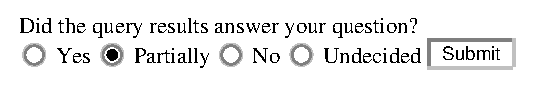
\includegraphics{example-figure.eps}
%%  \caption{An example of included Encapsulated PostScript (EPS).}
%% \label{fig:example-1}
%%\end{figure}
%
%\section{URLs}
%In this modern age, you may find that you wish to include URLs or pathnames
%which both tend to be long and hard for TeX to deal with because it doesn't
%know where to insert linebreaks. The ``{\tt url}'' package (loaded in the main
%uhtest.tex file) allows one to deal with these URLs. For example:
%
%Here is an URL which cannot be broken, leading to terrible output
%$<$http://www.hotwired.com/webmonkey/98/16/index2a.html$>$
%%% The "<>" have to be entered in math mode, that's where the "$"s come from.
%
%Using the package we get the much nicer \url{<http://www.hotwired.com/
%webmonkey/98/16/index2a.html>} which LaTeX can handle just fine. Even better,
%the parameter to {\tt $\backslash$url} can have spaces inserted anywhere so you
%can make the LaTeX source lines in your text editor wrap nicely.
%
%A few notes. It is recommended that you enclose your URLs in ``$<>$'' to ensure
%that any punctuation around the URL won't be confused as part of the URL. You
%can use URLs in your bibliography too (see the {\tt uhtest.bib} file for an
%example). Finally, if you need to use a tilde in your URL then things are a
%little trickier. One way to do it is like this:
%\url{<http://www.dartmouth.edu/}$\sim$\url{jonh/ff-cache/1.html>}. The {\tt
%$\backslash$url} style uses math mode internally, so we break the URL into two
%pieces, and stick a tilde from math mode inbetween the two parts.
%
%\section{Bibliography Citations}
%Citing references to your bibliography is easy \cite{lamport:latex}
%\cite{patashnik:bibtex}. First you build a BibTeX file which contains the
%records for all of the works you wish to cite. This file ends with a ``{\tt
%.bib}'' extension. Then in your body you use the ``{\tt $\backslash$cite}''
%command with the label you gave to the record in question. The final steps are: 
%run LaTeX once, run BibTeX, and then run LaTeX twice more. You should now have
%a bibliography that includes those citations.
%
%\chapter{Conclusion}
%
%This is going to be the chapter where I check the length of the page to make
%sure the bottom margin works out all right.  I hope you don't mind long
%annoying and useless paragraphs because you are sure to get a lot of them here!
%
%\section{Widgets}
%
%This is going to be the chapter where I check the length of the page
%to make sure the bottom margin works out all right.  I hope you don't
%mind long annoying and useless paragraphs because you are sure to get
%a lot of them here!
%
%\subsection{Sub-Widgets}
%
%This is going to be the chapter where I check the length of the page
%to make sure the bottom margin works out all right.  I hope you don't
%mind long annoying and useless paragraphs because you are sure to get
%a lot of them here!
%
%\subsubsection{Sub-Sub-Widgets}
%
%This is going to be the chapter where I check the length of the page
%to make sure the bottom margin works out all right.  I hope you don't
%mind long annoying and useless paragraphs because you are sure to get
%a lot of them here!
%
%\paragraph{Para-Widgets}
%
%This is going to be the chapter where I check the length of the page
%to make sure the bottom margin works out all right.  I hope you don't
%mind long annoying and useless paragraphs because you are sure to get
%a lot of them here!
%
%\subparagraph{Sub-Para-Widgets}
%
%This is going to be the chapter where I check the length of the page
%to make sure the bottom margin works out all right.  I hope you don't
%mind long annoying and useless paragraphs because you are sure to get
%a lot of them here!
%
%This is going to be the chapter where I check the length of the page
%to make sure the bottom margin works out all right.  I hope you don't
%mind long annoying and useless paragraphs because you are sure to get
%a lot of them here!
%
%This is going to be the chapter where I check the length of the page
%to make sure the bottom margin works out all right.  I hope you don't
%mind long annoying and useless paragraphs because you are sure to get
%a lot of them here!
%
%This is going to be the chapter where I check the length of the page
%to make sure the bottom margin works out all right.  I hope you don't
%mind long annoying and useless paragraphs because you are sure to get
%a lot of them here!
%
%This is going to be the chapter where I check the length of the page
%to make sure the bottom margin works out all right.  I hope you don't
%mind long annoying and useless paragraphs because you are sure to get
%a lot of them here!
%
%This is going to be the chapter where I check the length of the page
%to make sure the bottom margin works out all right.  I hope you don't
%mind long annoying and useless paragraphs because you are sure to get
%a lot of them here!
%
%This is going to be the chapter where I check the length of the page
%to make sure the bottom margin works out all right.  I hope you don't
%mind long annoying and useless paragraphs because you are sure to get
%a lot of them here!
%
%This is going to be the chapter where I check the length of the page
%to make sure the bottom margin works out all right.  I hope you don't
%mind long annoying and useless paragraphs because you are sure to get
%a lot of them here!
%
%This is going to be the chapter where I check the length of the page
%to make sure the bottom margin works out all right.  I hope you don't
%mind long annoying and useless paragraphs because you are sure to get
%a lot of them here!
%
%This is going to be the chapter where I check the length of the page
%to make sure the bottom margin works out all right.  I hope you don't
%mind long annoying and useless paragraphs because you are sure to get
%a lot of them here!
%
%This is going to be the chapter where I check the length of the page
%to make sure the bottom margin works out all right.  I hope you don't
%mind long annoying and useless paragraphs because you are sure to get
%a lot of them here!
%
%This is going to be the chapter where I check the length of the page
%to make sure the bottom margin works out all right.  I hope you don't
%mind long annoying and useless paragraphs because you are sure to get
%a lot of them here!
%
%This is going to be the chapter where I check the length of the page
%to make sure the bottom margin works out all right.  I hope you don't
%mind long annoying and useless paragraphs because you are sure to get
%a lot of them here!
%
%This is going to be the chapter where I check the length of the page
%to make sure the bottom margin works out all right.  I hope you don't
%mind long annoying and useless paragraphs because you are sure to get
%a lot of them here!
%
%This is going to be the chapter where I check the length of the page
%to make sure the bottom margin works out all right.  I hope you don't
%mind long annoying and useless paragraphs because you are sure to get
%a lot of them here!
%
%This is going to be the chapter where I check the length of the page
%to make sure the bottom margin works out all right.  I hope you don't
%mind long annoying and useless paragraphs because you are sure to get
%a lot of them here!
